  Im diesem Kapitel, soll auf die IT-Infrastruktur der \ac{ZKB} im Bereich der
  Web Applikationen eingegangen werden. Diese Informationen werden später dazu
  verwendet, um zu Prüfen, ob ein Java Web Framework den Ansprüchen der
  IT-Infrastruktur genügt. Die Informationen, welche hier beschrieben werden,
  stammen aus dem Handbuch der ZKB IT-Architektur, siehe
  \cite{ZkbHandbuchDerItArchitektur}. In der Abbildung
  \ref{img:infrastrukturZkb} ist die Standardkonfiguration, wie sie heute
  verwendet wird, ersichtlich.
  
  \begin{figure}[ht]
    \begin{center}
      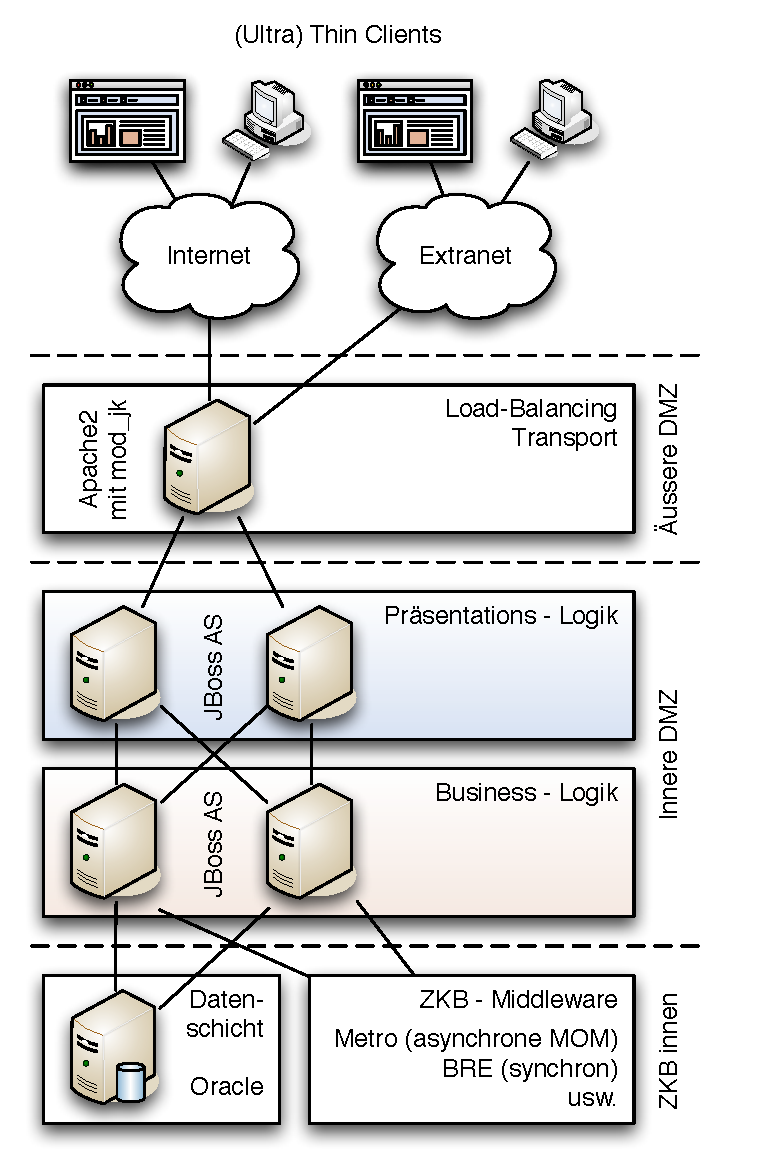
\includegraphics[width=0.87\textwidth]{./image/infrastrukturZkb.pdf}
      \caption{Architektur von Internet-Applikationen (nach
      \cite{ZkbHandbuchDerItArchitektur} S. 145)}
      \label{img:infrastrukturZkb}
    \end{center}
  \end{figure}
  
  \section{Java Runtime Environment}
  
  In allen Segmenten der Infrastruktur wird mindestens das \ac{JRE} von
  Oracle\footnote{ehemals Sun Microsystems} in der Version 1.5 zur Verfügung
  gestellt. An einigen stellen, zum Beispiel bei den Clients ist auch die
  Version 1.6 verfügbar. Diese Informationen beziehen sich auf den aktuellen
  Stand und können sich jederzeit ändern. Grundsätzlich wird nicht davon
  ausgegangen, dass ein Rückschritt in der Version vorgenommen wird, sondern
  das man gemäss der Evolution auf eine neuere Version wechselt.
  
  \section{Load-Balancing und Transport}
  
  Für das Load-Balancing und den Transport wird der Apache HTTP Server 2
  verwendet. Er gilt als anerkannter Standard und ist auf allen ZKB Plattformen
  verfügbar, siehe \cite{ZkbHandbuchDerItArchitektur} S. 146.
  
  Der Transport über \ac{HTTP} und \ac{HTTPS} gehört zu den Standardfunktionen
  des Apache HTTP Servers 2. Zudem können statische Daten direkt über den
  Apache HTTP Server 2 zur Verfügung gestellt werden, ohne das die
  Präsentations-Logik oder die Business-Logik damit belastet werden.
  
  Die Verbindung zur Präsentations-Logik und auch das Load-Balancing wird mit
  dem Modul\footnote{Der Apache HTTP Server 2 hat einen modularen Aufbau, womit
  er durch Module erweitert werden kann.} \(mod\_jk\)\footnote{Für
  Informationen zum Apache Tomcat Connector, siehe \cite{ModJk}} gemacht.
  
  \section{Präsentations-Logik}
  
  Für die Präsentations-Logik wird der Servlet/JSP Container JBoss
  Web\footnote{JBoss Web basiert auf Apache Tomcat 6.0 und implementiert die
  Standards Servlet 2.5 und JavaServer Pages 2.1, siehe \cite{JBossWeb}}
  verwendet, der ein Bestandteil des JBoss AS\footnote{JBoss AS steht für JBoss
  Application server, siehe \cite{JBossAS}} ist und auf der Open Source Software
  Apache Tomcat\footnote{Für mehr Informationen zu Apache Tomcat, siehe
  \cite{ApacheTomcat}} basiert. Der JBoss Web ist auch für die Verwaltung der
  User Sessions zuständig.
  
  Für die Präsentations-Logik wird eine komplette Instanz eines JBoss AS
  verwendet. Für die Skalierung der Web Applikation können weitere
  JBoss AS Instanzen dazugeschalten werden. In der standard Konfiguration sind
  es zwei.
  
  Für die Kommunikation zwischen der Präsentations-Logik und der Business-Logik
  werden Webservices auf der Basis von \ac{SOAP}, \ac{RMI} oder \ac{CORBA}
  verwendet. Es gibt auch eine \ac{ZKB} spezifische Lösung namens ZIP.net.
  
  Das für die Präsentations-Logik und die Business-Logik eigene JBoss AS
  Instazen verwendet werden, entspricht nicht ganz den Vorgaben, wie sie
  im Handbuch der IT-Architektur beschrieben sind, es wird aber in der Praxis
  oft so umgesetzt.
    
  \section{Business-Logik}
  
  Für die Business-Logik wird auch eine komplette Instanz eines JBoss AS
  verwendet. Für die Skalierung dieser Komponente können weitere JBoss AS
  Instanzen dazugeschalten werden. In der standard Konfiguration sind es zwei.
  
  Die Datenschicht wird über die Datenbankschnittstelle \ac{JDBC} angebunden.
  Der JBoss AS bietet für die meisten \ac{RDBMS} alles, was dafür benötigt
  wird. Es gibt auch die Konstellation, bei der ein \ac{ORM}, wie zum Beispiel
  Hibernate, verwendet wird.
  
  Die Kommunikation zwischen der Applikation und der ZKB spezifischen Middleware
  findet ebenfalls hier in der Business-Logik statt. Für die synchrone
  Kommunikation steht der \ac{BRE} zur Verfügung. Für die asynchrone
  Kommunikation gibt es Metro, was eine \ac{MOM} ist.
    
  \section{Datenschicht}
  
  Die Datenschicht wird meistens mit einem \ac{RDBMS} abgebildet. Normalerweise
  wird die Enterprise taugliche Lösung von Oracle eingesetzt. Je nach grösse
  der Applikation kann es sein, dass mehrere verschiedene \ac{RDBMS} zum Einsatz
  kommen.

